% ------------------------------------------------------------------------------
% section 01
% ------------------------------------------------------------------------------
\newpage
\section{Questions 1} 
\label{cha:q1}

\subsection[Q1-a]{Import data set to R assigning the type of each variable correctly}

We casted to factor both the string types ["Model", "SalesRegion"] and the very repetitive columns ["NumberofEngines", "EngineType"]. We considered casting also "ProductionYear", but in later calculation as the median was required, so we decided to leave as is (numerical). The code is shown below.

\begin{verbatim}
    air_data <- read.csv("./dataset.csv", sep=",", stringsAsFactors=TRUE)
    
    air_data <- air_data %>%
      rename(
        FC = FuelConsumption.L.h.,
        HM = HourlyMaintenance...,
        Price = Price...
      )
      
    to_factors <- c("Model", "NumberofEngines", "EngineType", "SalesRegion")
    
    for (col in to_factors) {
      air_data[[col]] <- as.factor(air_data[[col]])
    }
\end{verbatim}

\subsection[Q1-b]{Summarize the variables Price, Fuel Consumption first for the all data and then for the groups of Engine Type}

We reported the result of the summaries of both Price and Fuel Consuption in the tables \ref{tab:q10} and \ref{tab:q11}, while an histogram is in figure \ref{fig:q10}

\begin{table}[H]
    \centering
    \begin{tabular}{CCCCCC}
        \hline
        Min. & 1st Qu. & Median & Mean & 3rd Qu. & Max. \\
        \hline
        145815 & 14096814 & 83921914 & 198833650 & 384323881 & 978213229 \\
        \hline
    \end{tabular}
    \caption{Price}
    \label{tab:q10}
\end{table}

\begin{table}[H]
    \centering
    \begin{tabular}{CCCCCC}
        \hline
        Min. & 1st Qu. & Median & Mean & 3rd Qu. & Max. \\
        \hline
        2.00 & 5.95 & 9.82 & 12.08 & 13.47 & 49.97 \\
        \hline
    \end{tabular}
    \caption{Fuel Consumption (FC)}
    \label{tab:q11}
\end{table}

\begin{figure}[H]
    \centering
    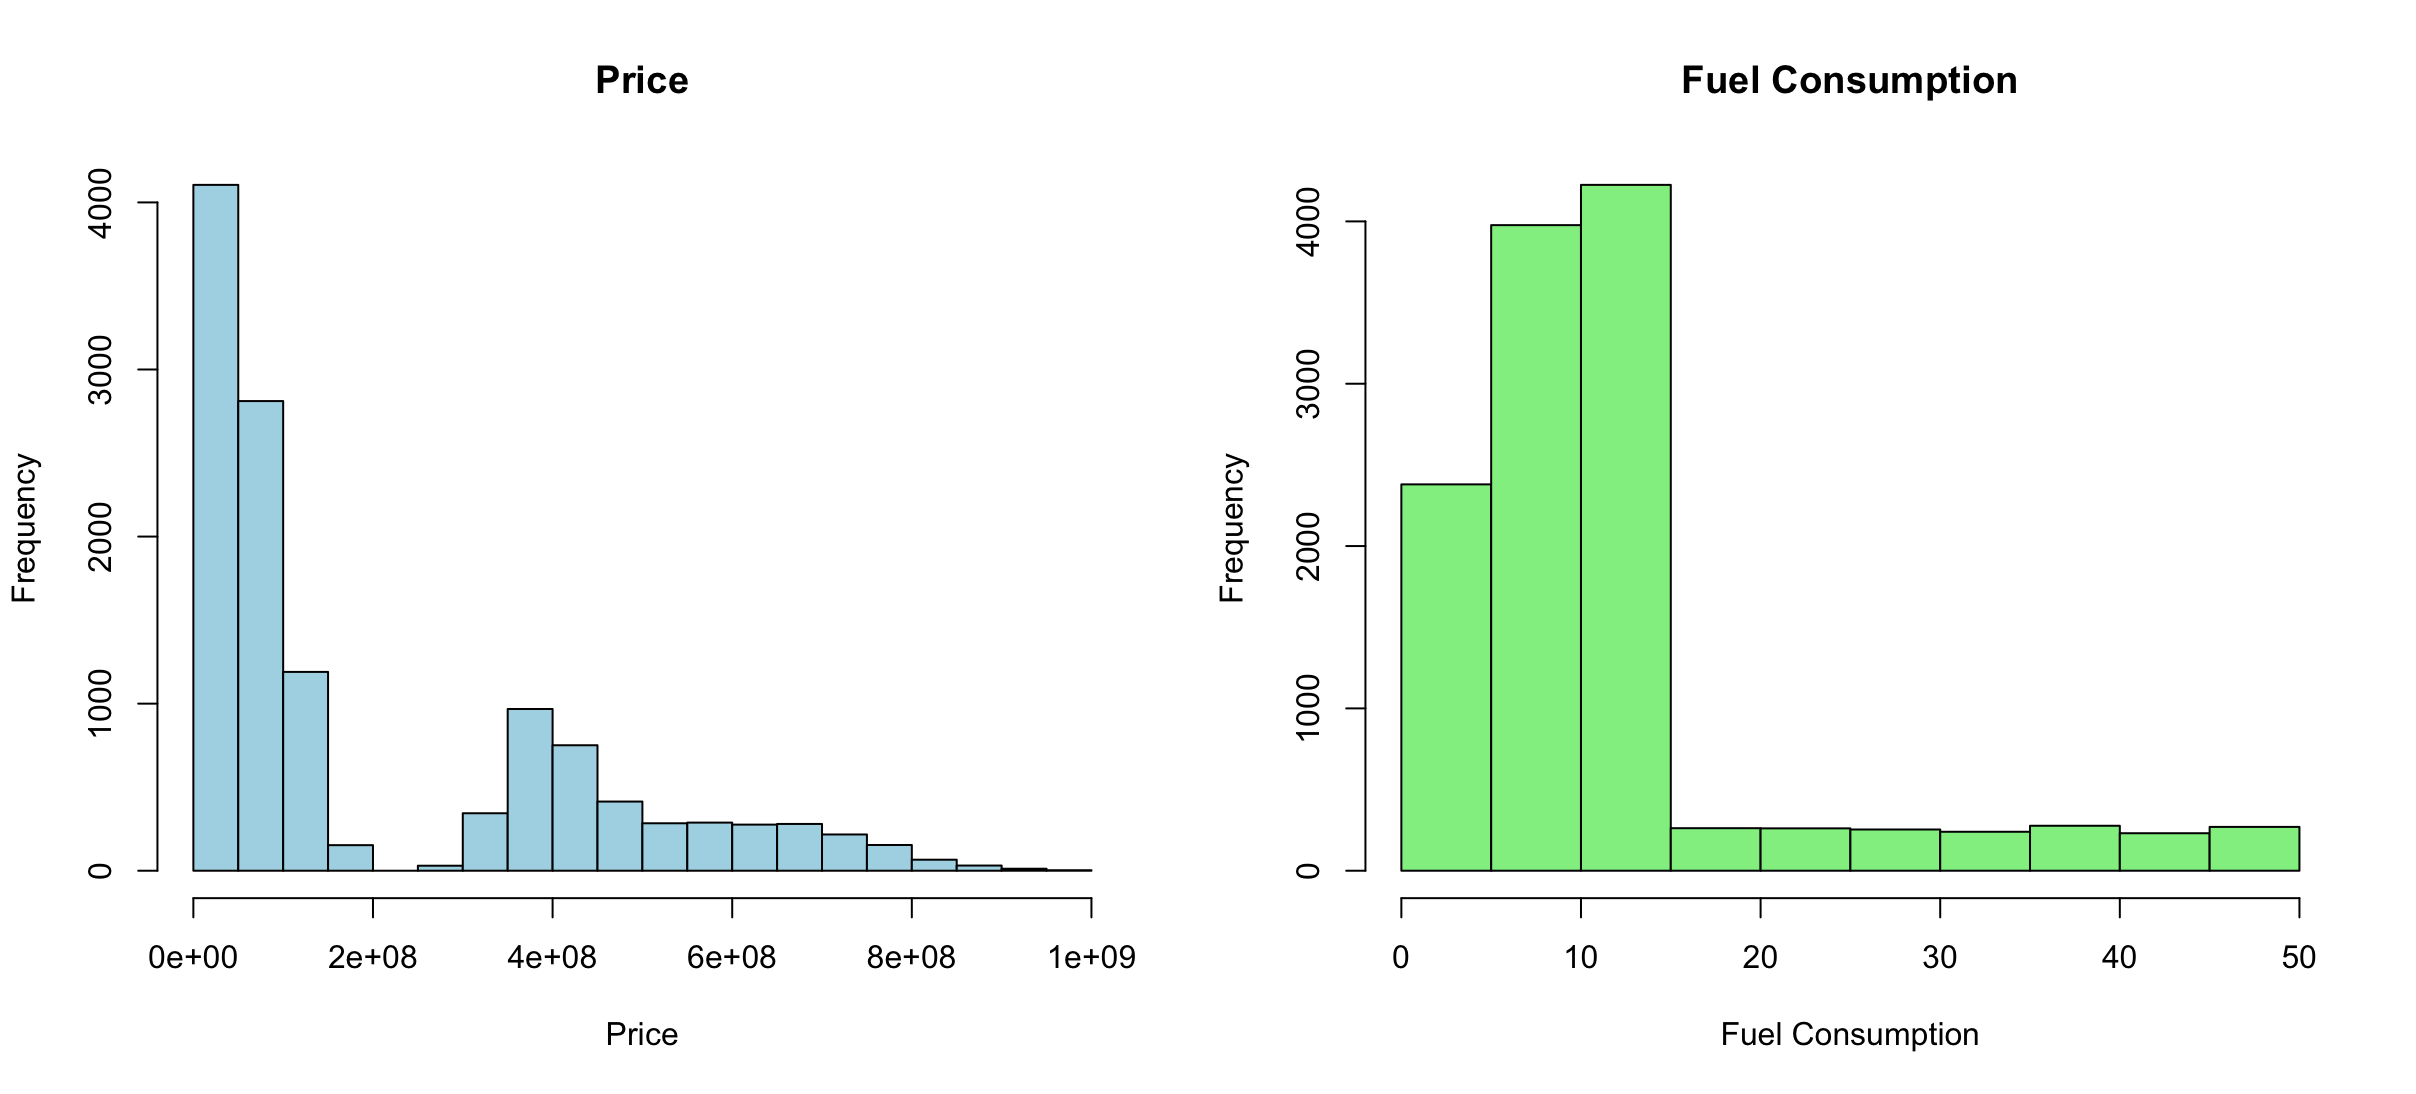
\includegraphics[width=\figsizetext]{Q1/01-summary-all-data.png}
    \caption{Histograms} 
    \label{fig:q10}
\end{figure}

Here are the same summaries but based on the Engine Type (Table \ref{tab:q12} and Figure \ref{fig:q11}).

\begin{table}[H]
    \centering
    \resizebox{\textwidth}{!}{
    \begin{tabular}{lrrrrrrrrrrr}
    \hline
    EngineType & Price\_Mean & Price\_SD & Price\_Median & Price\_Min & Price\_Max & FC\_Mean & FC\_SD & FC\_Median & FC\_Min & FC\_Max & n \\
    \hline
    Piston & 279405. & 77369. & 251474. & 145815. & 561279. & 30.1 & 11.6 & 29.9 & 10.0 & 50.0 & 2039 \\
    Turbofan & 237995200. & 231292861. & 108876395. & 8150222. & 978213229. & 8.52 & 3.75 & 8.53 & 2.0 & 15.0 & 10338 \\
    \hline
    \end{tabular}%
    }
    \caption{Summary by Model}
    \label{tab:q12}
\end{table}

\begin{figure}[H]
    \centering
    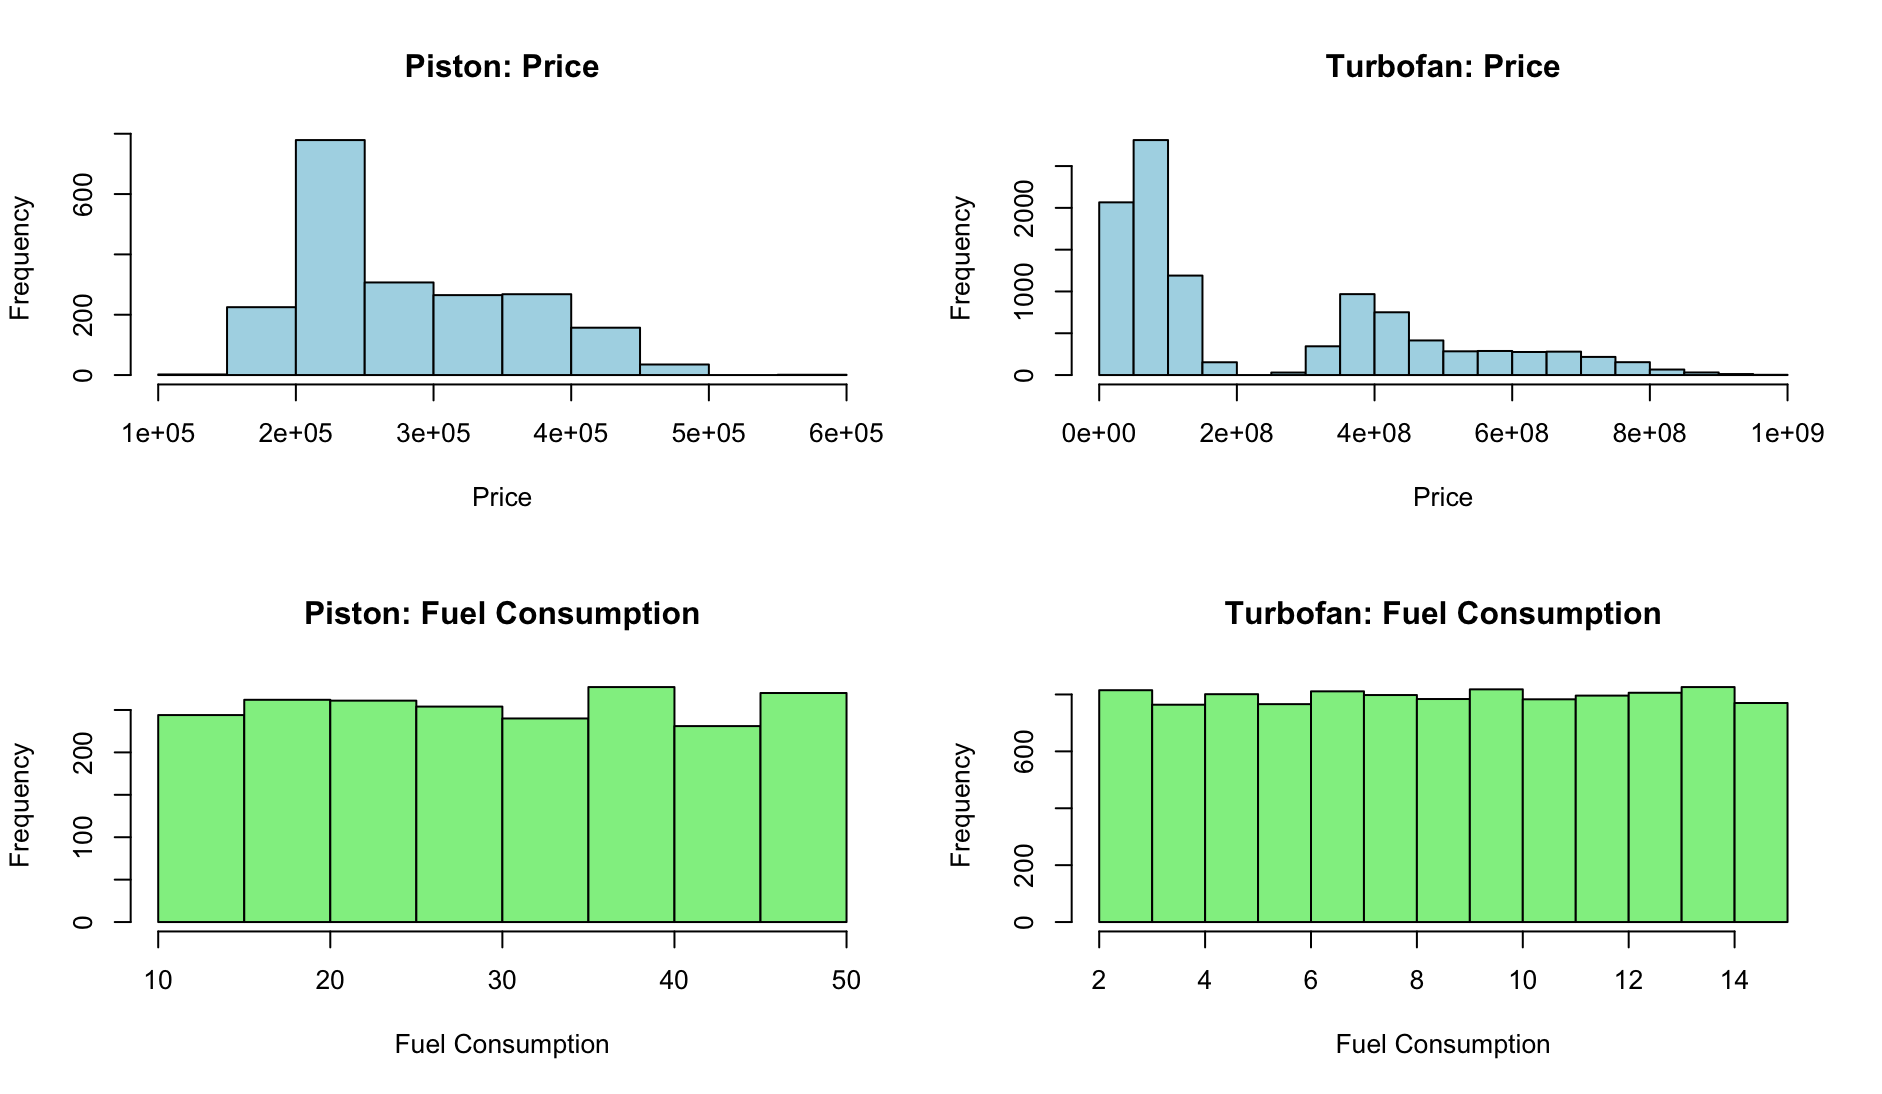
\includegraphics[width=\figsizetext]{Q1/02-summary-by-type.png}
    \caption{Summary distributions by Model} 
    \label{fig:q11}
\end{figure}

\subsection[Q1-c]{Test whether Fuel Consumption is affected from the Engine Type of the plane. Check the assumptions and visualize the relationship between these two characteristics} 

\begin{figure}[H]
    \centering
    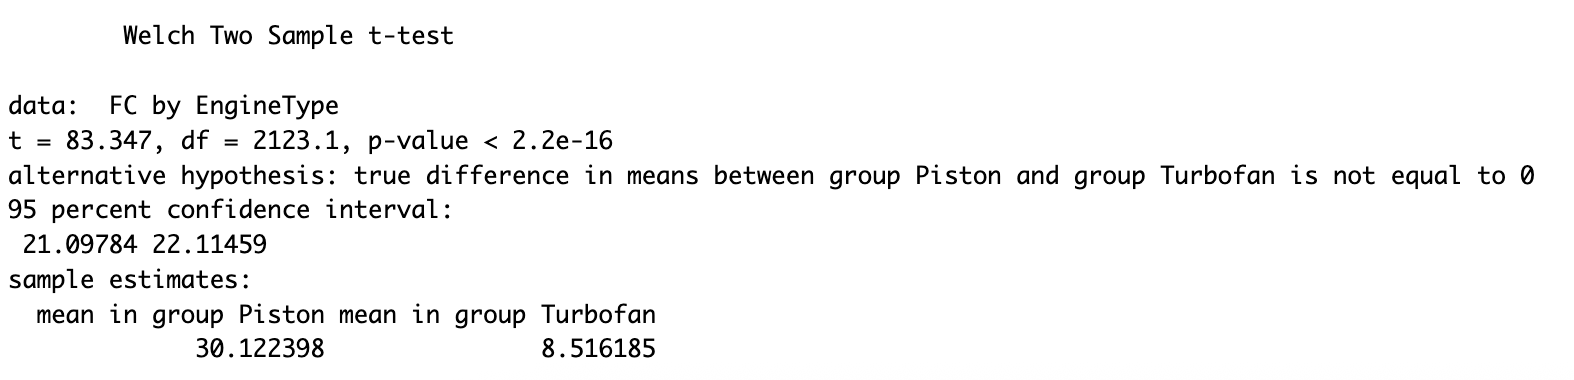
\includegraphics[width=\figsizetext]{Q1/05-ttest-by-engine.png}
    \caption{T-test results for Fuel Consumption by Engine Type} 
    \label{fig:q14}
\end{figure}

We performed a t-test and obtained a p-value, the results can be found in the figure  \ref{fig:q14}. Since the p-value is $<$ 0.05, we reject the null hypothesis and conclude that there is a significant difference in mean fuel consumption between the engine types. Furthermore we used a visual interpretation to be sure about the result as the number of observation made the test not very significant (figures \ref{fig:q12} and \ref{fig:q13}).

\begin{figure}[H]
    \centering
    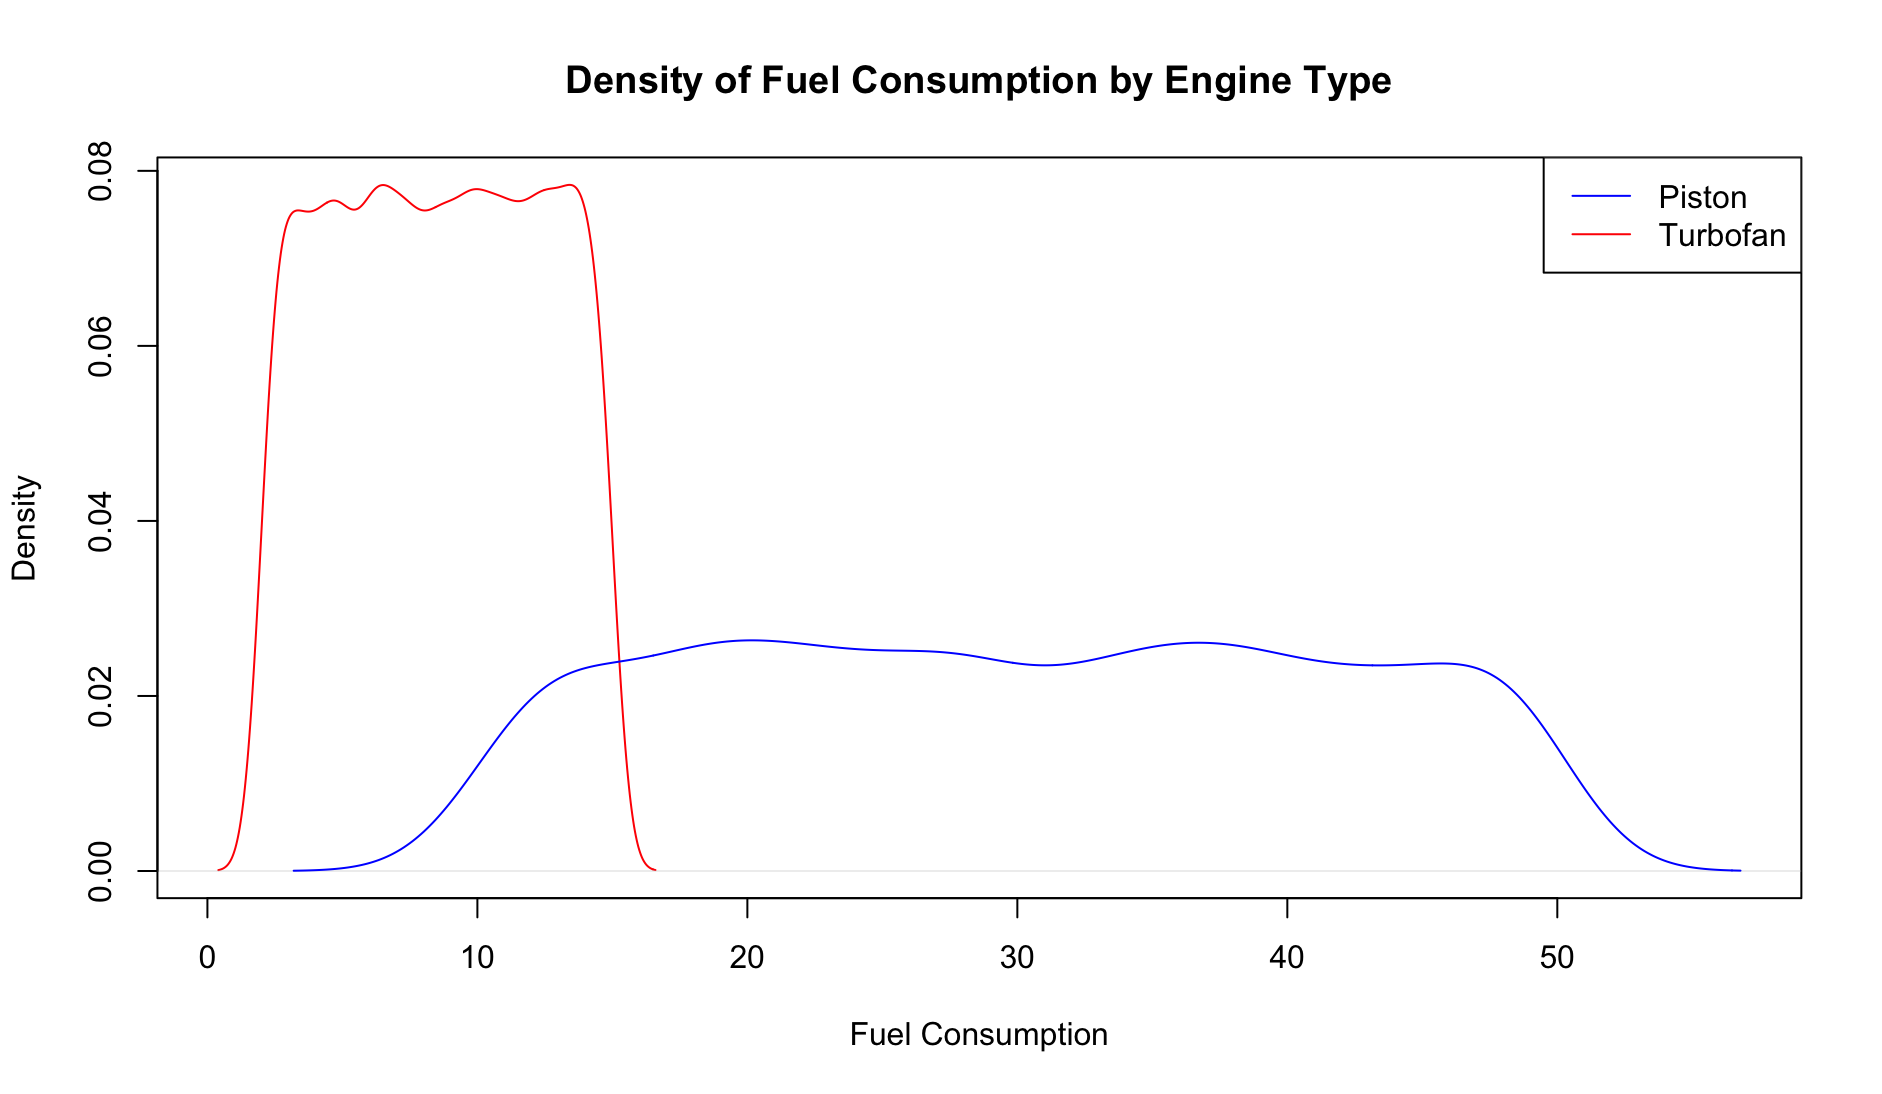
\includegraphics[width=\figsizetext]{Q1/03-summary-by-type2.png}
    \caption{Comparing distributions}
    \label{fig:q12}
\end{figure}

\begin{figure}[H]
    \centering
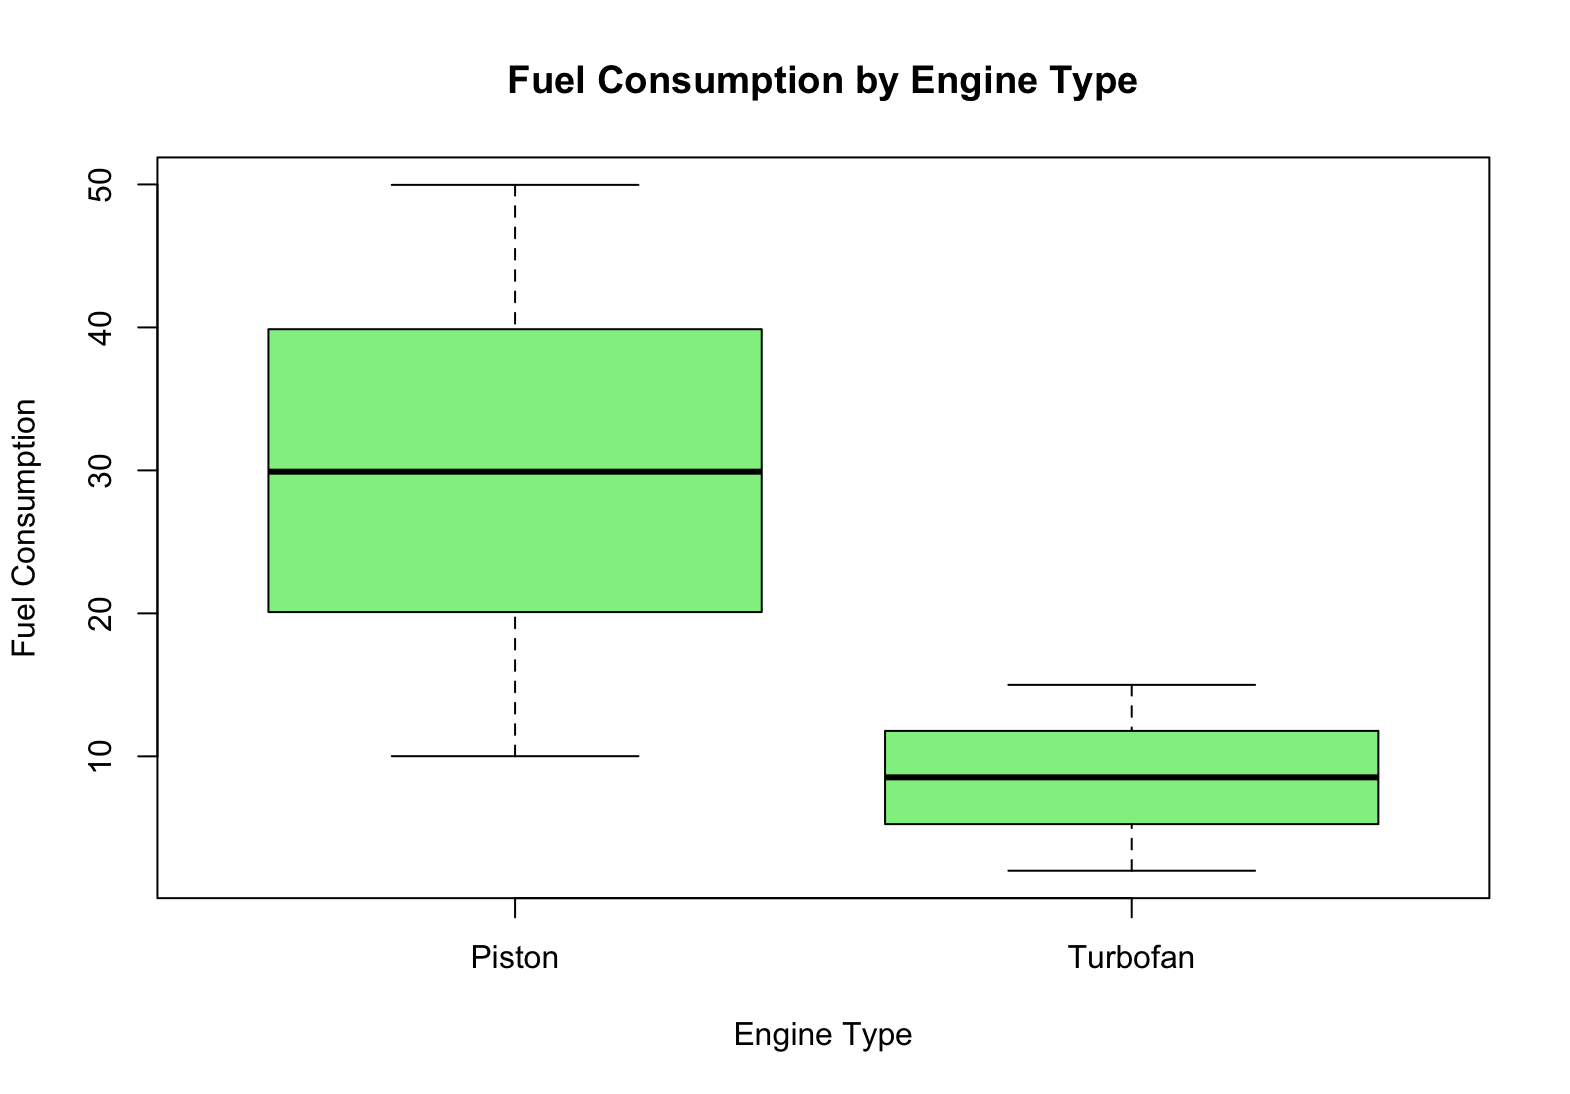
\includegraphics[width=\figsizetext]{Q1/04-boxplot-by-type.png}
    \caption{Boxplot is best for comparing a continuous variable across categories} 
    \label{fig:q13}
\end{figure}

\subsubsection*{Test assumptions}

\begin{itemize}
    \item We checked for normality (Shapiro-Wilk) and homogeneity of variances (Levene's test). Because the sample size is large (N $>$ 5000), 
    the normality test is overly sensitive, but the large sample size allows us to rely on the Central Limit Theorem.
    \item Variance was addressed by using the default robust t-test in R (Welch's t-test).
\end{itemize}

\subsection[Q1-d]{Construct 95\% confidence intervals for the mean of two groups and interpret them} % Promoted to \subsection[Q1-]

\begin{itemize}
    \item We are 95\% confident 
    that the true population mean of FC for Piston engines lies within that interval \textbf{(29.61919, 30.62560)}.
    \item Similarly, the 95\% CI 
    for Turbofan is \textbf{(8.443816, 8.588554)}.
\end{itemize}

The two intervals do NOT overlap. This provides visual evidence that the mean Fuel Consumption differs significantly between the two engine types.

\subsection[Q1-e]{Check the association between Model and Sales Region in the whole sample using proper method and interpret your findings}

To check the association between the 2 categories we used the chi square as the two types of variable needed it. The code is shown below.

\begin{verbatim}
    table_model_region <- table(air_data$Model, air_data$SalesRegion)
    chisq_result <- chisq.test(table_model_region)
\end{verbatim}

The obtained p-value $>$ 0.05 ($\sim$0.73), so we fail to reject the null hypothesis and conclude that there is no statistically significant association between Model and Sales Region. The airplane models are distributed similarly across sales regions.

\subsection[Q1-f]{Filter your data only considering $Bombardier CRJ200$ and $Cessna 172$ model airplanes}

Here we applied a simple filter and removed the empty buckets. this way we obtained a clean dataset with only the 2 models.

\begin{verbatim}
    filtered_air_data <- air_data |>
      filter(Model %in% c("$Bombardier CRJ200$", "$Cessna 172$")) |>
      droplevels()
\end{verbatim}

\subsection[Q1-g]{Check the distribution of Price across two categories of Engine type (You can apply transformation if you think it is required)}

Here we applied a transformation to the price (log) since it appeared to be completely left-skewed. visually we can clearly conclude that there is a significant difference of Price between the two types of Engines. Data can be visualized in figures \ref{fig:q15} and \ref{fig:q16}

\begin{figure}[H]
    \centering
    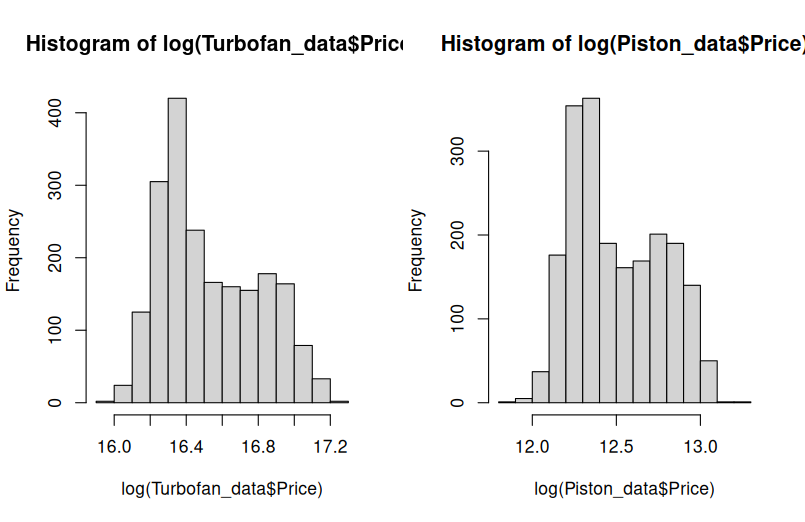
\includegraphics[width=\figsizetext]{Q1/06-boxplot-logprice-by-type.png}
    \caption{Histogram of Log Price by Engine Type} 
    \label{fig:q15}
\end{figure}

\begin{figure}[H]
    \centering
    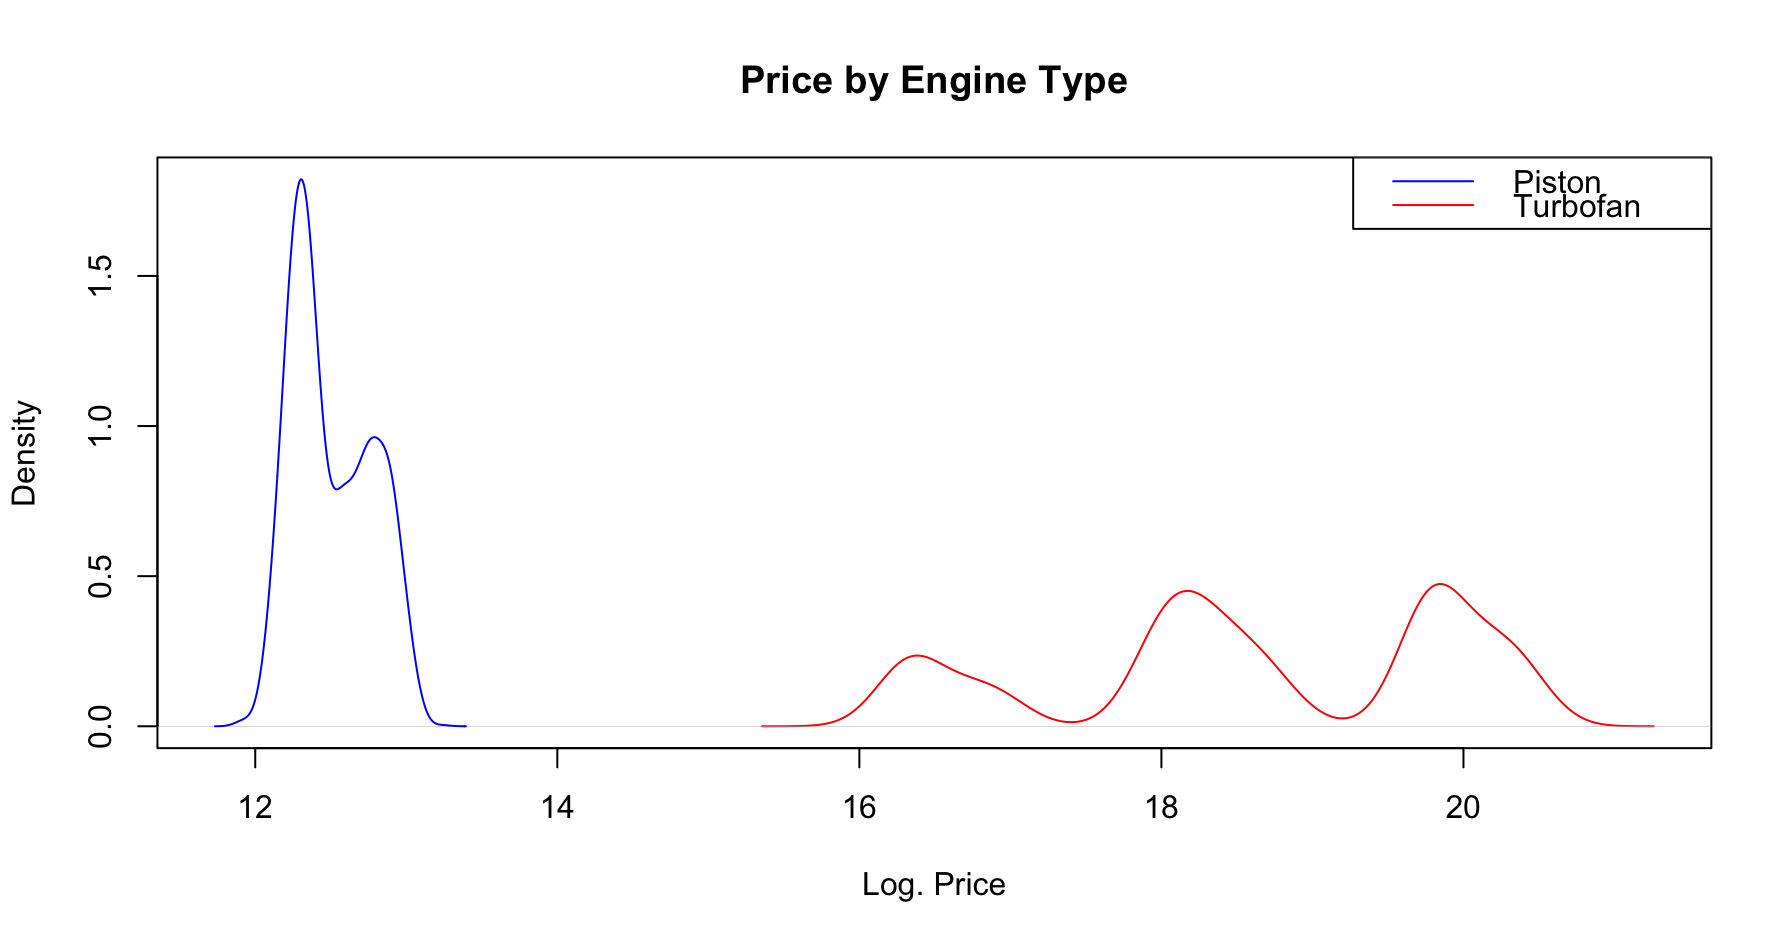
\includegraphics[width=\figsizetext]{Q1/07-plot-logprice-by-type.png}
    \caption{Distribution plot of Log Price by Engine Type} 
    \label{fig:q16}
\end{figure}

\subsection[Q1-h]{Categorize the variable Price into two categories as "low" and "High" by cutting from the median and save it as a new variable into your data frame}

To compute the categorization of price we first calculated the median and then applied it to a new variable: $Price\_Category$.

\begin{verbatim}
    median_price <- median(filtered_air_data$Price, na.rm = TRUE)
    filtered_air_data$Price_Category <- factor(
      ifelse(filtered_air_data$Price > median_price, "High", "Low")
    )
\end{verbatim}

\subsection[Q1-i]{Cross classify model and price categories and interpret the conditional probabilities}

Row proportions P(PriceCategory $\vert$ Model) table shows (table \ref{tab:q13}), for each model, what proportion of its airplanes fall into "Low" vs "High" price. Since $Bombardier CRJ200$ (Turbofan) has much higher prices than $Cessna 172$ (Piston), we expect nearly all $Bombardier CRJ200$ to be in the "High" category and nearly all $Cessna 172$ to be in the "Low" category. Nevertheless, using the median as a separator, some $Bombardier CRJ200$ still fell into the "low" category because the number of the first model is slightly higher than that of the second model..

\begin{table}[H]
    \centering
    \begin{tabular}{lPP}
        \hline
        & High & Low \\
        \hline
        $Bombardier CRJ200$ & 0.997074598 & 0.002925402 \\
        $Cessna 172$ & 0.000000000 & 1.000000000 \\
        \hline
    \end{tabular}
    \caption{Conditional probabilities: P(PriceCategory $\vert$ Model) - row proportions}
    \label{tab:q13}
\end{table}

Column proportions P(Model $\vert$ PriceCategory) table shows (table \ref{tab:q14}), for each price category, what proportion belongs to each model. This table confirms further the hypothesis of association between the model and price. The "low" category is dominated by $Cessna 172$ and the "High" category by $Bombardier CRJ200$, so it confirms a strong association between airplane model and price 

\begin{table}[H]
    \centering
    \begin{tabular}{lPP}
        \hline
        & High & Low \\
        \hline
        $Bombardier CRJ200$ & 1.000000000 & 0.002933985 \\
        $Cessna 172$ & 0.000000000 & 0.997066015 \\
        \hline
    \end{tabular}
    \caption{Conditional probabilities: P(Model $\vert$ PriceCategory) - column proportions}
    \label{tab:q14}
\end{table}

\subsection[Q1-j]{Is there an association between the model of the airplane and its price level. Analyze it by using proper statistical method} 

we applied the chi square test and obtained a p-value as a result.

\begin{verbatim}
    test_model_price <- chisq.test(cross_model_price)
\end{verbatim}

The p-value $<$ 0.05, so we reject the null hypothesis and conclude that there is a statistically significant association between airplane model and price level. Given that $Bombardier CRJ200$ (Turbofan) costs millions while $Cessna 172$ (Piston) costs hundreds of thousands, we expect a very small p-value, confirming a strong association.

\subsection[Q1-k]{Cross classify the variables Model and Sales region. Interpret the conditional probabilities and then test whether there is an association between these two characteristics}

P(SalesRegion $\vert$ Model) (row proportions, table \ref{tab:q15}) shows the distribution of sales regions for each model. Both models have similar proportions across regions, so we conclude that the sales region is independent of the model.

\begin{table}[H]
    \centering
    \resizebox{\textwidth}{!}{
        \begin{tabular}{lrrrrrr}
            \hline
            & Africa & Asia & Australia & Europe & North America & South America \\
            \hline
            $Bombardier CRJ200$ & 0.1843003 & 0.1628474 & 0.1604096 & 0.1589469 & 0.1638225 & 0.1696733 \\
            $Cessna 172$ & 0.1652771 & 0.1726336 & 0.1696910 & 0.1765571 & 0.1574301 & 0.1584110 \\
            \hline
        \end{tabular}%
    }
    \caption{Conditional probabilities: P(SalesRegion $\vert$ Model)}
    \label{tab:q15}
\end{table}

P(Model $\vert$ SalesRegion) (column proportions, table \ref{tab:q16}) shows, within each region, what share belongs to each model. Both models appear in roughly equal proportions within every region, so this supports our independence assumption.

\begin{table}[H]
    \centering
    \resizebox{\textwidth}{!}{
        \begin{tabular}{lrrrrrr}
            \hline
            & Africa & Asia & Australia & Europe & North America & South America \\
            \hline
            $Bombardier CRJ200$ & 0.5286713 & 0.4868805 & 0.4874074 & 0.4752187 & 0.5114155 & 0.5186289 \\
            $Cessna 172$ & 0.4713287 & 0.5131195 & 0.5125926 & 0.5247813 & 0.4885845 & 0.4813711 \\
            \hline
        \end{tabular}%
    }
    \caption{Conditional probabilities: P(Model $\vert$ SalesRegion)}
    \label{tab:q16}
\end{table}

We applied a chi square test to further test the hypothesis. As expected, p-value $>$ 0.05 ($\sim$0.29), so we fail to reject the null hypothesis and conclude there is no significant association. The two models are sold in similar proportions across regions.